\chapter{Оптимизация параметров}\label{optimization}
Код FAINA позволяет не только расчитывать излучение заданных источников, но и фитировать наблюдательные данные модельными, подбирая необходимые параметры. Реализованы методы оптимизации, пригодные для произвольного числа параметров и широкого класса моделей источников. В качестве целевой функции используется взвешенная сумма квадратов отклонений по всем наблюдательным точкам $f = \sum \frac{(F_i - F_{obs,i})^2}{\sigma_i^2}$, где $F_i$ - расчетная спектральная плотность потока излучения, $F_{obs,i}$ - наблюдаемая спектральная плотность потока излучения, $\sigma_i$ - её погрешность. В текущей версии учитывается лишь погрешность измеряемого потока, ширина бина и неопределенность энергии, на которой принят сигнал не учитываются.

Реализованные методы оптимизации делятся на два типа - те, которые рассматривают излучение в один момент времени, либо постоянные во времени, и те, которые учитывают эволюцию источников и используют наблюдения в разные моменты времени. В последнем случае пользователю необходимо самостоятельно указывать, как меняются параметры источника со временем, см. раздел \ref{timeDependentSource}.

\section{Фитирование источников, не зависящих от времени}
Для фитирования постоянных во времени кривых блеска предназначен абстрактный класс RadiationOptimizer. В нем определена виртуальныя функция optimize(double* vector, bool* optPar, double* energy, double* observedFlux, double* observedError, int Ne, RadiationSource* source), которая и производит процесс оптимизации. Входными параметрами являются: vector - массив подбираемых параметров, в который будет записан результат работы программы, optPar - массив булевских переменных, определяющих оптимизировать соответствующий параметр, или считать его фиксированным, energy - массив энергий, на которых производились наблюдения, observedFlux - соответствующие наблюдаемые потоки в единицах $\text{см}^{-2}\text{с}^{-1}$, Ne - количество наблюдательных точек, source - источник излучения. Функция изменения параметров источника source->resetParameters, описанная в разделе \ref{sourcesSection}, должна быть согласована с массивом оптимизируемых параметров vector, так как в процессе оптимизации он будет передаваться в нее в качестве аргумента.

В коде реализованы два наследника класса RadiationOptimazer: GridEnumRadiationOptimizer - производящий поиск минимума простым перебором по сетке параметров с заданным количеством распределенных равномерно логарифмически точек, и GradientDescentRadiationOptimizer - в котором минимум находится методом градиентного спуска. Эти два класса полезно использовать совместно, используя результат работы первого как начальную точку для второго. Схема насследования классов оптимизаторов показана на рисунке \ref{radiationOptimizer}, а список их публичных методов приведен в Таблице \ref{RadiationOptimizerMethods}. Реализованные методы оптимизации применимы для всех описанных выше типов источников и видов электромагнитного излучения.
\begin{figure}
	\centering
	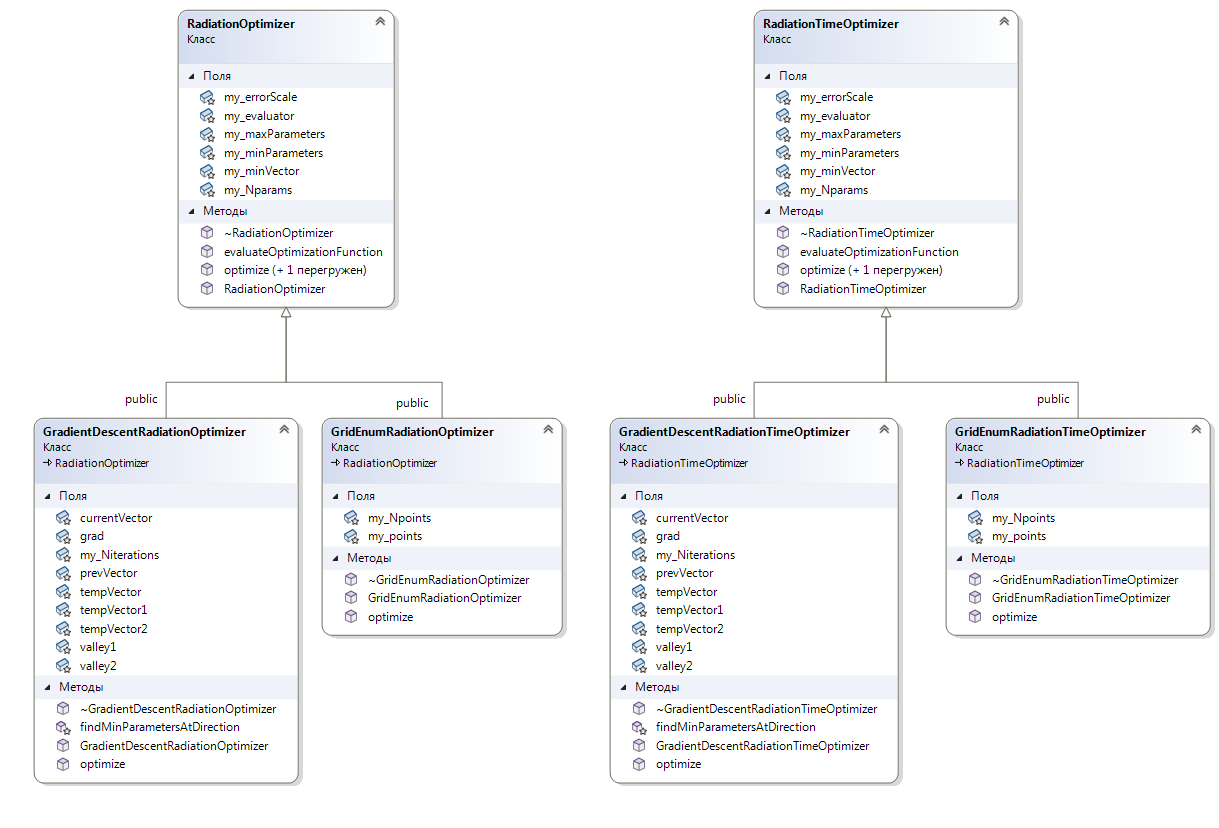
\includegraphics[width=11.5 cm]{./fig/radiationOptimizer.png} 
	\caption{Схема наследования классов оптимизаторов}
	\label{radiationOptimizer}
\end{figure}

\begin{small}
	\topcaption{Публичные методы классов оптимизаторов параметров источников }
	\label{RadiationOptimizerMethods}
	\begin{xtabular}{|p{0.41\textwidth}|p{0.59\textwidth}|}
		\hline
		\textbf{RadiationOptimizer} & абстрактный класс для оптимизации параметров источника \\
		\hline
		evaluateOptimizationFunction( const double* vector, double* energy, double* observedFlux, double* observedError, int Ne, RadiationSource* source) & вычисляет целевую функцию - взвешенную сумму квадратов ошибок во всех наблюдательных точках $f = \sum \frac{(F_i - F_{obs,i})^2}{\sigma_i^2}$, где $F_i$ - расчетная спектральная плотность потока излучения, $F_{obs,i}$ - наблюдаемая спектральная плотность потока излучения, $\sigma_i$ - её погрешность\\
		\hline
		optimize( double* vector, bool* optPar, double* energy, double* observedFlux, double* observedError, int Ne, RadiationSource* source) & функция, осуществляющая оптимизацию, принимает на вход массив подбираемых параметров, в который будет записан результат, массив булевских переменных, определяющих оптимизировать соответствующий параметр, или считать его фиксированным, массив энергий, на которых производились наблюдения, соответствующие наблюдаемые потоки в единицах $\text{см}^{-2}\text{с}^{-1}$, погрешности измерения потоков, количество наблюдательных точек, и источник излучения.\\
		\hline
		optimize( double* vector, bool* optPar, double* energy, double* observedFlux, int Ne, RadiationSource* source) & функция, осуществляющая оптимизацию, в случае не заданных наблюдательных ошибок. В таком случае ошибки у всех точек считаются равными елинице и веса всех ошибок в целевой функции оказываются равными\\
		\hline
		\textbf{GridEnumRadiationOptimizer} & класс предназначенный для оптимизации параметров с помощью перебора по сетке\\
		\hline
		GridEnumRadiationOptimizer( RadiationEvaluator* evaluator, const double* minParameters, const double* maxParameters, int Nparams, const int* Npoints) & конструктор, создает экземпляр класса с указанным вычислителем излучения, минимальными и максимальными значениями оптимизируемых параметров, количеством этих параметров и массивом с количеством перебираемых точек по каждому параметру. При переборе точки будут распределены логарифмически равномерно по оси.\\
		\hline
		\textbf{GradientDescentRadiationOptimizer} & класс, предназначенный для оптимизации параметров методом градиентного спуска\\
		\hline
		GradientDescentRadiationOptimizer( RadiationEvaluator* evaluator, const double* minParameters, const double* maxParameters, int Nparams, int Niterations) & конструктор, создает экземпляр класса с указанным вычислителем излучения, минимальными и максимальными значеними оптимизируемых параметров, количеством этих параметров и максимальным количеством итераций градиентного спуска\\
		\hline		
	\end{xtabular}
\end{small}

Пример фитирования параметров источника по наблюдательным данным приведен в функции fitCSS161010withPowerLawDistribition в файле main.cpp. Следуя авторам работы \cite{Coppejans2020} произведем расчет синхротронного излучения источника с учетом самопоглощения, считая функцию распределения электронов чисто степенной с показателем 3.6. Но мы не будем накладывать дополнительную связь на параметры и предполагать равенство распределения энергии между магнитным полем и ускоренными частицами, вместо этого магнитное поле и концентрация электронов будут независимыми параметрами.

Подберем параметры Быстрого Оптического Голубого Транзиента CSS161010 на 98 день после вспышки на основе радиоизлучения. Зададим параметры источника на основе дынных статьи \cite{Coppejans2020}, которые будут использоваться в качестве начального приближения, а так же расстояние до него.
\begin{lstlisting}[language=c++]
    double electronConcentration = 25;
    double B = 0.6;
    double R = 1.4E17;
    double fraction = 0.5;
    const double distance = 150 * 1E6 * parsec;
\end{lstlisting}
Далее зададим степенное распределение электронов, с показателем 3.6 и источник в форме плоского диска, перпендикулярного лучу зрения, и вычислитель синхротронного излучения.
\begin{lstlisting}[language=c++]
    double Emin = me_c2;
    double Emax = 10000 * me_c2;
    double index = 3.6;
	
    SynchrotronEvaluator* synchrotronEvaluator = new 
	    SynchrotronEvaluator(200, Emin, Emax);
    MassiveParticlePowerLawDistribution* electrons = new 
	    MassiveParticlePowerLawDistribution(massElectron, index, 
	    Emin, electronConcentration);
    SimpleFlatSource* source = new 
	    SimpleFlatSource(electrons, B, 1.0, R, fraction*R, distance);
\end{lstlisting}
Теперь определим вектор оптимизируемых параметров - это размер, магнитное поле, концентрация электронов и доля толщины, показывающая какю долю от радиуса диска составляет его толщина. И именно такие параметры ожидает функция resetParameters у источника SimpleFlatSource. Так же нужно указать минимальные и максимальные значения параметров, которые ограничат область поиска. Максимальные значения так же будут использоваться как константы нормировки.
\begin{lstlisting}[language=c++]
    const int Nparams = 4;
    double minParameters[Nparams] = { 1E17, 0.01, 0.5, 0.1 };
    double maxParameters[Nparams] = { 2E17, 10, 200, 1.0 };
    double vector[Nparams] = { R, B, electronConcentration, fraction};
    for (int i = 0; i < Nparams; ++i) {
	    vector[i] = vector[i] / maxParameters[i];
    }
\end{lstlisting}
Зададим наблюдательные данные, которые и будем фитировать. Обратите внимание, что частоты нужно перевести в энергии, а спектральную плотность потока - в энергетическую (в единицы $\text{см}^{-2}\text{с}^{-1}$).
\begin{lstlisting}[language=c++]
    const int Nenergy1 = 4;
    double energy1[Nenergy1] = { 1.5E9*hplank, 3.0E9 * hplank, 
    	6.1E9 * hplank, 9.8E9 * hplank };
    double observedFlux[Nenergy1] = { 1.5/(hplank*1E26), 
    	4.3/(hplank*1E26), 6.1/(hplank*1E26), 4.2 /(hplank*1E26)};
    double observedError[Nenergy1] = { 0.1 / (hplank * 1E26), 
    	0.2/(hplank*1E26), 0.3/(hplank*1E26), 0.2/(hplank*1E26)};
\end{lstlisting}
Далее создадим два оптимизатора - действющий перебором и градиентым спуском, и применим их последовательно. Так же укажем количество точек для перебора и то, что оптимизируем все параметры.
\begin{lstlisting}[language=c++]
    bool optPar[Nparams] = { true, true, true, true };
    int Niterations = 20;
    int Npoints[Nparams] = { 10,10,10,10 };
    
    RadiationOptimizer* enumOptimizer = new GridEnumRadiationOptimizer(
        synchrotronEvaluator,minParameters,maxParameters,Nparams,Npoints);
    RadiationOptimizer* gradientOptimizer = new 
        GradientDescentRadiationOptimizer(synchrotronEvaluator, 
        minParameters, maxParameters, Nparams, Niterations);
\end{lstlisting}
Применим функцию optimize у последовательно у обоих оптимизаторов. Сначала перебором найдем начальное приближение, потом уточним результат с помощью градиентного спуска, и изменим параметры источника на оптимальные
\begin{lstlisting}[language=c++]
    enumOptimizer->optimize(vector, optPar, energy1, observedFlux, 
        observedError, Nenergy1, source);
    gradientOptimizer->optimize(vector, optPar, energy1, observedFlux, 
        observedError, Nenergy1, source);
    source->resetParameters(vector, maxParameters);
\end{lstlisting}
Полученные в результате оптимизации парметры источника равны: радиус диска $R = 1.8\times10^17 \text{ см}$, магнитное поле $B = 1.6 \text{ Гс}$, концентрация электронов $n = 2.3 \text{ см}^{-3}$, доля толщины $fraction = 0.54 $. Значение целевой функции $f \approx 50$. Модельный спектр излучения  с данными параметрами и наблюдательные данные изображены на рисунке \ref{synchrotron1}.
\begin{figure}
	\centering
	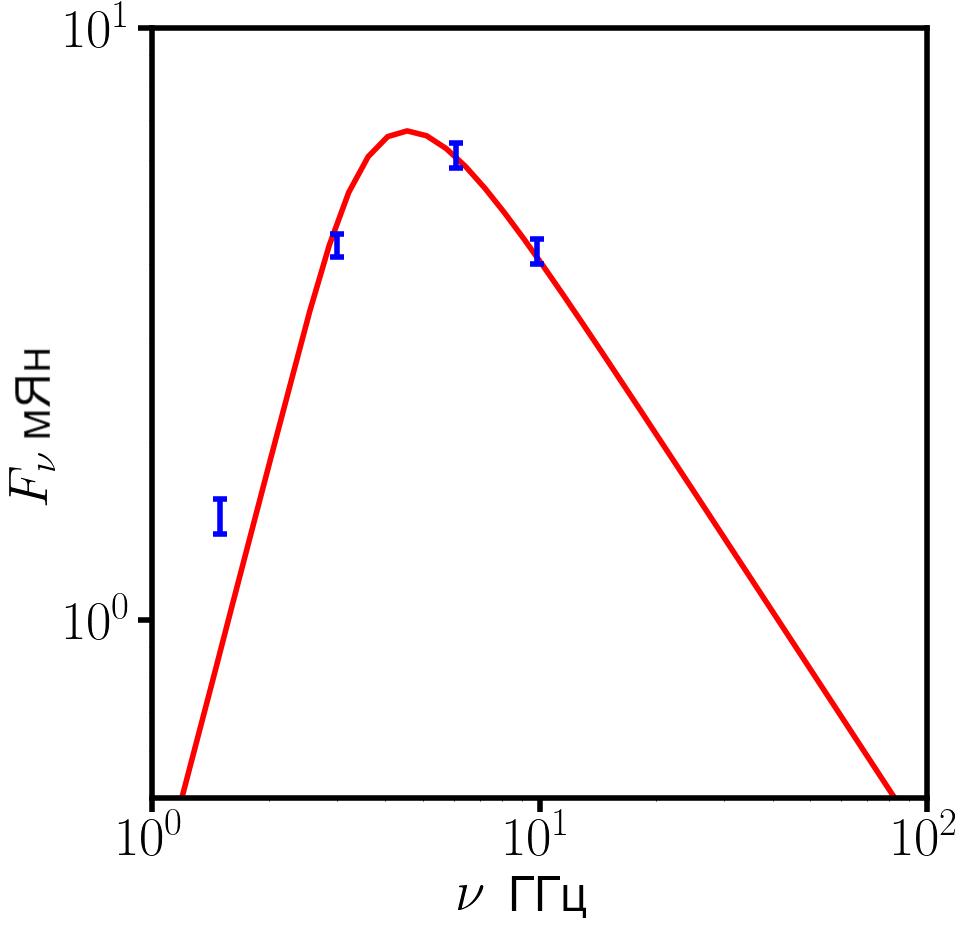
\includegraphics[width=12.5 cm]{./fig/synchrotron1.png} 
	\caption{Наблюдаемый и расчетный спектр радиоизлучения объекта CSS161010 на 98 день после вспышки}
	\label{synchrotron1}
\end{figure}
\section{Фитирование источников, зависящих от времени}
Для фитирования постоянных во времени кривых блеска изменяющихся во времени предназначен абстрактный класс RadiationTimeOptimizer. В нем определена виртуальныя функция optimize(double* vector, bool* optPar, double** energy, double** observedFLux, double** observedError, int* Ne, int Ntimes, double* times, RadiationTimeDependentSource* source), которая и выполняет оптимизацию. Так же как и в случае не зависящей от времени оптимизации она принимает на вход массив параметров, массив булевских переменных, и наблюдательные данные. Но наблюдательные данные теперь представляют собой двумерные массивы (причем количество заданных точек в разные моменты времени так же может быть разным). Так же нужно указать количество серий измерений во времени и соответствующие им времена. Исследуемый источник должен относиться к классу зависящих от времени источников.

Как и ранее, в коде реализованы два наследника класса RadiationTimeOptimazer: GridEnumRadiationTimeOptimizer - для поиска минимума перебором, и GradientDescentRadiationTimeOptimizer - в котором минимум находится методом градиентного спуска. Схема насследования классов оптимизаторов показана на рисунке \ref{radiationOptimizerTime}, а список их публичных методов приведен в Таблице \ref{RadiationTimeOptimizerMethods}.
\begin{figure}
	\centering
	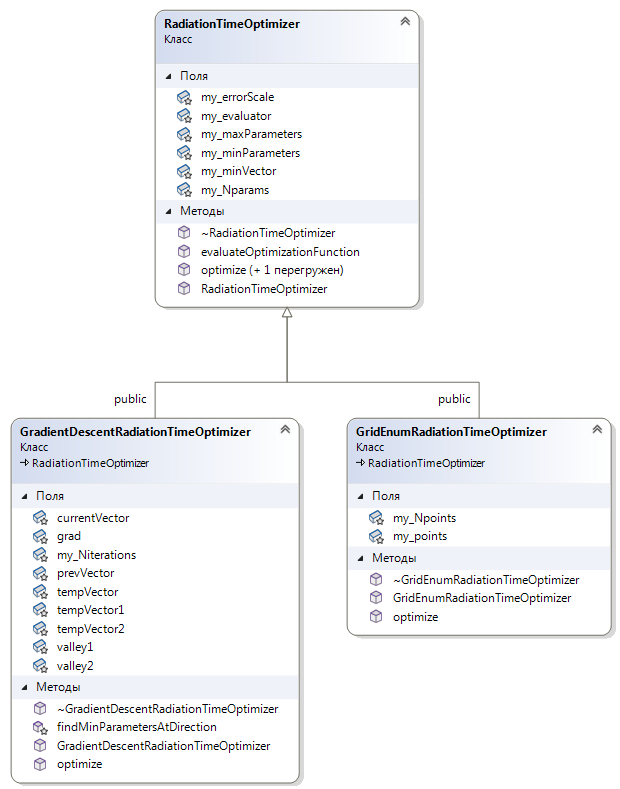
\includegraphics[width=10.5 cm]{./fig/radiationOptimizerTime.png} 
	\caption{Схема наследования классов оптимизаторов, учитывающих переменность источников}
	\label{radiationOptimizerTime}
\end{figure}

\begin{small}
	\topcaption{Публичные методы классов оптимизаторов параметров переменных во времени источников }
	\label{RadiationTimeOptimizerMethods}
	\begin{xtabular}{|p{0.5\textwidth}|p{0.5\textwidth}|}
		\hline
		\textbf{RadiationTimeOptimizer} & абстрактный класс, предназначенный для оптимизации параметров зависящих от времени источников\\
		\hline
		evaluateOptimizationFunction( const double* vector, double** energy, double** observedFlux, double** observedError, int* Ne, int Ntimes, double* times, RadiationTimeDependentSource* source) & вычисляет целевую функцию - взвешенную сумму квадратов ошибок во всех наблюдательных точках во все моменты времени $f = \sum \frac{(F_i - F_{obs,i})^2}{\sigma_i^2}$, где $F_i$ - расчетная спектральная плотность потока излучения, $F_{obs,i}$ - наблюдаемая спектральная плотность потока излучения, $\sigma_i$ - её погрешность\\
		\hline
		optimize (double* vector, bool* optPar, double** energy, double** observedFLux, double** observedError, int* Ne, int Ntimes, double* times, RadiationTimeDependentSource* source) & функция, осуществляющая оптимизацию, принимает на вход массив подбираемых параметров, в который будет записан результат, массив булевских переменных, определяющих оптимизировать соответствующий параметр, или считать его фиксированным, двумерные массивы энергий, на которых производились наблюдения, соответствующих энергиям наблюдаемых потоков в единицах $\text{см}^{-2}\text{с}^{-1}$, погрешности наблюдаемых потоков, массив количества наблюдательных точек в каждый момент времени, количество моментов времени, когда производились измерения, соответствующие времена и переменный источник излучения.\\
		\hline
		optimize(double* vector, bool* optPar, double** energy, double** observedFlux, int* Ne, int Ntimes, double* times, RadiationTimeDependentSource* source) & функция, осуществляющая оптимизацию, в случае не заданных наблюдательных ошибок. В таком случае ошибки у всех точек считаются равными елинице и веса всех ошибок в целевой функции оказываются равными\\
		\hline
		\textbf{GridEnumRadiationTimeOptimizer} & класс, предназначенный для оптимизации параметров переменных источников с помощью перебора по сетке\\
		\hline
		GridEnumRadiationTimeOptimizer( RadiationEvaluator* evaluator, const double* minParameters, const double* maxParameters, int Nparams, const int* Npoints) & конструктор, создает экземпляр класса с указанным вычислителем излучения, минимальными и максимальными значениями оптимизируемых параметров, количеством этих параметров и массивом с количеством перебираемых точек по каждому параметру. При переборе точки будут распределены логарифмически равномерно.\\
		\hline
		\textbf{GradientDescentRadiationTimeOptimizer} & класс, предназначенный для оптимизации параметров переменных источников методом градиентного спуска\\
		\hline
		GradientDescentRadiationTimeOptimizer( RadiationEvaluator* evaluator, const double* minParameters, const double* maxParameters, int Nparams, int Niterations) & конструктор, создает экземпляр класса с указанным вычислителем излучения, минимальными и максимальными значеними оптимизируемых параметров, количеством этих параметров и максимальным количеством итераций градиентного спуска\\
		\hline		
\end{xtabular}
\end{small}